\begin{figure}[H]
\centering
\includegraphics[page=8,width=0.44\textwidth]{\FCNCFigures/tthML/showFake/faketau/prefit/NOMINAL/reg2l1tau1bnj_vetobtagwp70_highmet/tau_pt_0.pdf}
%\put(-100, 140){\textbf{(a1)}}
%\put(-120, 130){\footnotesize{$2l1tau1b$}}
\includegraphics[page=8,width=0.44\textwidth]{\FCNCFigures/tthML/showFake/faketau/prefit/NOMINAL/reg2l1tau2bnj_vetobtagwp70_highmet/tau_pt_0.pdf}
%\put(-100, 140){\textbf{(a2)}}
%\put(-120, 130){\footnotesize{$2l1tau2b$}}

\includegraphics[page=8,width=0.44\textwidth]{\FCNCFigures/tthML/showFake/faketau/prefit/NOMINAL/reg1l1tau2b2j_os_vetobtagwp70_highmet/tau_pt_0.pdf}
%\put(-100, 140){\textbf{(b1)}}
%\put(-120, 130){\footnotesize{$1l1tau2b2j OS$}}
\includegraphics[page=8,width=0.44\textwidth]{\FCNCFigures/tthML/showFake/faketau/prefit/NOMINAL/reg1l1tau2b3j_os_vetobtagwp70_highmet/tau_pt_0.pdf}
%\put(-100, 140){\textbf{(b2)}}
%\put(-120, 130){\footnotesize{$1l1tau2b3j OS$}}

\includegraphics[page=8,width=0.44\textwidth]{\FCNCFigures/tthML/showFake/faketau/prefit/NOMINAL/reg1l1tau2b2j_ss_vetobtagwp70_highmet/tau_pt_0.pdf}
%\put(-100, 140){\textbf{(c1)}}
%\put(-120, 130){\footnotesize{$1l1tau2b2j SS$}}
\includegraphics[page=8,width=0.44\textwidth]{\FCNCFigures/tthML/showFake/faketau/prefit/NOMINAL/reg1l1tau2b3j_ss_vetobtagwp70_highmet/tau_pt_0.pdf}
%\put(-100, 140){\textbf{(c2)}}
%\put(-120, 130){\footnotesize{$1l1tau2b3j SS$}}
\caption{ The distributions of $\tau$ $\pt$ used to calibrate the fake taus in the control regions of leptonic channel. Only statistical uncertainties are being shown. Underflow and overflow bins are included respectively in the first and last bins. The real tau contributions shown from ttbar and other MC including diboson, single top, and V+jets.}
\label{fig:wjet_pt_CR}
\end{figure}
